%% 02_problema_necesidad/contenido.tex -- Subdocumento 2 del Formulario T-7.
%% Generado desde lafrox-markdown/02_problema_necesidad/LAFROX-Subdocumento2.md
\tikzset{
  lfxNode/.style={draw=lafroxFuerte, rounded corners=2pt, minimum width=2.4cm, minimum height=1.05cm, align=center, fill=lafroxBg, font=\small\sffamily, thick},
  lfxCrit/.style={draw=lafroxFuerte, rounded corners=2pt, minimum width=2.4cm, minimum height=1.05cm, align=center, fill=lafroxTenue, font=\small\sffamily, thick},
  lfxDec/.style={draw=lafroxFuerte, rounded corners=6pt, minimum width=2.2cm, minimum height=1.05cm, align=center, fill=white, font=\footnotesize\sffamily, thick},
  lfxArrow/.style={draw=lafroxFuerte, ->, >=stealth, thick},
  lfxDash/.style={draw=lafroxGris, dashed, ->, >=stealth, thick}
}

\setcounter{chapter}{1}
\chapter{Introducción al Problema y Necesidad}

El presente subdocumento expone el diagnóstico integral, operacional y estratégico de Distribuidora Puelche S.A. en el marco del caso. Se analiza la estructura de su modelo logístico actual (\textit{AS-IS}), caracterizado por una profunda fragmentación de datos, procesos manuales en terreno y desacoples entre la promesa comercial y la capacidad física de distribución.

Este capítulo establece la línea base conceptual y cuantitativa para el resto de la propuesta: fundamenta los requerimientos funcionales y el alcance técnico, define los requerimientos no funcionales y de resiliencia, y delimita las restricciones operativas que condicionan la planificación de la implantación. El catálogo pormenorizado de requerimientos del cliente, el registro extendido de supuestos y exclusiones, y el inventario nominal de actores y sistemas legados se presentan en los Anexos~2.1 a 2.3 de este subdocumento.

\section{Resumen Ejecutivo del problema}

Distribuidora Puelche S.A. enfrenta una crisis de eficiencia y competitividad operacional producto de la obsolescencia y desarticulación de su ecosistema informático. Su operación integra los centros de distribución de Talca y Concepción y tres plataformas de \textit{cross-docking}. La flota considera 42 camiones propios y 54 de diez transportistas. En reparto trabajan 84 conductores y peonetas propios y cerca de 160 conductores de transportistas, y se atienden 14.200 puntos de entrega. La operación actual exhibe un índice de entrega a tiempo y completa (OTIF) de 82,4 \%, frente a una referencia de 95 \% (Distribuidora Puelche S.A., 2026c, cap. 7, tabla 7.1, p. 11). Por tanto, el 17,6 \% de los despachos no llega completo y a tiempo. Esto deteriora la relación con el canal tradicional y pone en riesgo a la principal cadena de supermercados, que representa el 11 \% de la venta y fija nuevas condiciones desde enero de 2029 (Distribuidora Puelche S.A., 2026c, cap. 1, p. 3).

La raíz del problema no reside en un único sistema defectuoso, sino en un tejido heterogéneo y desconectado: un ERP implantado en 2017 cuyos módulos satélites de preventa fueron abandonados por su proveedor, un WMS de 2013 con soporte discontinuado y procesos críticos gobernados mediante planillas de cálculo y papel. Esta desconexión tecnológica genera tres impactos críticos inmediatos:

\begin{enumerate}
  \item \textbf{Vulnerabilidad sanitaria y regulatoria:} El retiro preventivo de marzo de 2026 demoró 9 días y alcanzó 4.800 kg del lote 24-0217, con una pérdida directa de dinero. El proveedor suspendió a Puelche por seis meses de su lista de distribuidores autorizados; ese proveedor representa el 6\% de las ventas. En el producto involucrado, el 41\% de las recepciones no registraba lote en el sistema.
  \item \textbf{Fricción comercial y quiebre de preventa:} El 7,8 \% de las líneas de pedido tomadas en terreno presenta quiebre de stock, pues los 62 preventistas operan a ciegas mediante una aplicación móvil obsoleta sin visibilidad de inventario ni crédito en tiempo real.
  \item \textbf{Opacidad financiera y diferencias de rendición sin investigar:} La empresa subsidia entregas ineficientes bajo un prorrateo de costo de servir estático fijado en 2016. La rendición manual diferida del efectivo genera diferencias no conciliadas; además, el 1,1\% mensual de las guías de despacho se extravía o queda ilegible; ante un reclamo de entrega no recibida, encontrar la guía toma en promedio 12 días.
\end{enumerate}

Estas brechas establecen la necesidad que debe abordar la oferta: recuperar trazabilidad de lote, hacer confiable la promesa de entrega, disminuir la pérdida de información en terreno y disponer de una base objetiva para gestionar el costo de servir. El Capítulo 3 define la solución y el alcance que responderán a estas necesidades.

\section{Comprensión del problema y de la necesidad}

Esta sección descompone el problema en tres dimensiones, lo sitúa en su contexto operacional, normativo y estacional, y registra las tensiones entre áreas que la solución debe resolver.

\subsection{Los tres problemas entrelazados}

El caso pide distinguir tres problemas entrelazados (Distribuidora Puelche S.A., 2026c, cap. 19, p. 35). La problemática de Puelche se descompone en esas tres dimensiones, que se retroalimentan:

\begin{enumerate}
  \item \textbf{Habilitación sanitaria y comercial comprometida:} El cumplimiento del Reglamento Sanitario de los Alimentos (Decreto 977) exige el control riguroso de la cadena de frío (congelados a $-$18\,°C o menos; la cámara de congelado de Talca opera a $-$22\,°C) (Ministerio de Salud, 1996) y la trazabilidad bidireccional inmediata de lotes. En la actualidad, el registro de temperatura es discontinuo e instrumentalizado por el propio conductor, sin alarmas automáticas ante excursiones térmicas. Al recibir mercadería de los 180 proveedores, el personal revisa las fechas de vencimiento por muestreo y registra el lote de manera incompleta, en un campo de texto libre. La trazabilidad depende del papel de recepción y de la memoria de quienes despacharon, sin estar disponible de forma consultable en los sistemas. Esta carencia expone a Puelche a sanciones de la autoridad sanitaria, que ya observó la ausencia de registro continuo de temperatura en su última fiscalización. También le impide acreditar ante el proveedor de lácteos la capacidad de trazabilidad que este exige para restablecer la relación tras la suspensión, que vence en septiembre de 2026.
  \item \textbf{Pérdida de competitividad del servicio:} El nivel de servicio actual (OTIF 82,4 \% y \textit{fill rate} 91,3 \%) está lejos de las referencias de 95 \% y 97 \% que el caso asocia a esos indicadores. Además, la principal cadena exigirá desde enero de 2029 pedido electrónico, aviso de despacho, ventana de entrega de 30 minutos con penalización y prueba de entrega digital. Hoy Puelche entrega entre las 08:00 y las 18:00. Los clientes del canal tradicional (11.600 almacenes) y \textit{food service} (2.100 puntos) enfrentan faltantes y retrasos. La falta de visibilidad en preventa y la rigidez de las rutas provocan reentregas equivalentes al 4,2\% de las entregas. Sobre la referencia de 1.400 entregas diarias, ello equivale a aproximadamente 59 reentregas al día (1.400 $\times$ 0,042 = 58,8).
  \item \textbf{Desconocimiento estructural del costo de servir:} La fijación de precios y márgenes se calcula sobre un costo de transporte promedio estático que data de 2016. Puelche desconoce el costo real de atender a cada cliente, subsidiando rutas rurales remotas de baja densidad a expensas de clientes urbanos de alta rotación. La ocupación promedio de la flota es 68\% y cae a 41\% en días de baja utilización. La rotación anual de preparadores de pedidos alcanza 38\%, lo que incrementa el esfuerzo de capacitación e induce errores recurrentes en el armado de pedidos.
\end{enumerate}

\subsection{Contexto operacional, normativo y estacionalidad}

La comprensión del negocio de Distribuidora Puelche S.A. exige interpretar sus restricciones regulatorias y sectoriales bajo el marco jurídico chileno vigente:

\begin{itemize}
  \item \textbf{Reglamento Sanitario de los Alimentos (Decreto 977/1996 del Ministerio de Salud):} (Ministerio de Salud, 1996). Obliga a mantener registros inalterables de temperatura en alimentos congelados (temperatura $\le$ $-$18\,°C) y a ejecutar procedimientos de retiro de mercado (\textit{recall}) en plazos expeditos ante sospecha de contaminación microbiológica o química.
  \item \textbf{Documentos Tributarios Electrónicos (DTE - SII):} (Servicio de Impuestos Internos, 2024). La Guía de Despacho Electrónica (GDE) rige el traslado legal de mercaderías. El acuse de recibo electrónico con constancia de entrega conforme o recepción con mermas es el instrumento probatorio que otorga mérito ejecutivo para la cobranza comercial y el cómputo del crédito fiscal IVA.
  \item \textbf{Normativa laboral de transportes:} El artículo 25 bis del Código del Trabajo regula la jornada y los descansos de los choferes de vehículos de carga terrestre interurbana. Estas condiciones deben considerarse al planificar las rutas a las que resulte aplicable esta regulación (Ministerio del Trabajo y Previsión Social, 2002, art. 25 bis).
  \item \textbf{Ley 21.719 de Protección de Datos Personales:} La entrada en vigencia de la ley está fijada para el 1 de diciembre de 2026 (Ley N.º 21.719, 2024, art. primero transitorio). Por ello, Puelche debe preparar el tratamiento de información comercial y comportamiento financiero de los almaceneros, y los controles telemáticos deben respetar la proporcionalidad laboral y la restricción del caso sobre cámaras y GPS.
  \item \textbf{Estándares sectoriales GS1 y EDI:} (GS1 Chile, 2020). Demanda la adopción de identificadores universales (GTIN para productos, GLN para puntos de entrega, GS1-128 para unidades logísticas de carga) e intercambio electrónico de datos (EDI) para órdenes de compra, avisos de despacho (DESADV) y facturación electrónica con el gran retail chileno.
\end{itemize}

A este marco se añade el impacto crítico de la \textbf{estacionalidad}, durante las tres primeras semanas de septiembre el volumen diario casi se duplica, de $\approx$ 1.400 a $\approx$ 2.600 entregas (Distribuidora Puelche S.A., 2026c, sección B.2, pp. 38--39). Este pico satura la ventana de preparación nocturna (22:00 a 06:00 hrs) y genera congestión severa en la ventana crítica de despacho matinal (05:30 a 07:00 hrs). Un dimensionamiento informático o de flota calculado para promedios mensuales colapsa inevitablemente en este período. Similar tensión ocurre en diciembre y durante los cierres mensuales, mientras que en invierno los caminos rurales empeoran y alargan los tramos sin señal, que en rutas de hasta 240 km ya llegan a dos horas.

\subsection{Arbitraje de tensiones operacionales y comerciales}

Las entrevistas de levantamiento del caso (Distribuidora Puelche S.A., 2026c, cap. 8, pp. 13--17) muestran contradicciones estructurales entre las distintas gerencias de Puelche. Estas tensiones no constituyen discrepancias accidentales, sino el reflejo de objetivos locales descoordinados que exigen una decisión antes de diseñar la solución. Para cada tensión se indica la decisión que la necesidad requiere:

\begin{enumerate}
  \item \textbf{Promesa de entrega (Comercial contra Operaciones):} La Gerencia Comercial busca captar clientes prometiendo entregas en 24 horas a todo evento. La Gerencia de Operaciones afirma que tal promesa es materialmente imposible en la flota actual y genera frustración y reclamos. \textbf{Decisión que requiere la necesidad:} una promesa segmentada y viable: 24 horas para clientes urbanos con pedidos ingresados antes del corte de las 14:00, y 48 horas para clientes rurales, periféricos o abastecidos mediante \textit{cross-docking}. Cómo se informa la promesa al cliente se desarrolla en el Subdocumento 3.
  \item \textbf{Control de cadena de frío (Calidad contra Operaciones):} La Jefa de Calidad exige que cualquier excursión térmica fuera de norma bloquee automáticamente el producto para entrega. Operaciones y los choferes argumentan que bloqueos ciegos obligan a retornar camiones cargados y provocan pérdidas catastróficas. \textbf{Decisión que requiere la necesidad:} un control térmico graduado: las excursiones menores y transitorias (apertura de puertas durante la descarga) justifican una advertencia, y solo las críticas y sostenidas (sobre el umbral del RSA) justifican retener el lote; la decisión final sobre el producto es de Calidad (Anexo~2.2, S-04). El mecanismo de alerta y retención se desarrolla en el Subdocumento 3.
  \item \textbf{Gestión del efectivo (Finanzas contra Comercial):} Finanzas exige erradicar el efectivo y exigir transferencias o prepagos para evitar pérdidas. Comercial sostiene que exigir bancarización liquidará al canal tradicional. \textbf{Decisión que requiere la necesidad:} se respeta el pago en efectivo del canal tradicional, sin exigir al almacenero un dispositivo propio. La necesidad es que cada cobro quede asociado a su entrega y que la diferencia de rendición pueda rastrearse por entrega, en vez de detectarse al día siguiente. El mecanismo de registro, comprobante y cuadratura se desarrolla en el Subdocumento 3.
  \item \textbf{Nube y cortes de enlace (Jefe de TI contra la operación):} El jefe de TI prefiere todo en la nube y él mismo explica por qué la operación no puede depender de ella: la fibra se corta cuatro veces al año, Concepción no tiene respaldo y las plataformas de cross-docking operan solo con red móvil. \textbf{Decisión que requiere la necesidad:} la preferencia por la nube es admisible solo si la operación no depende del enlace. Cada centro de distribución debe poder recibir, preparar y despachar durante al menos 24 horas sin enlace, y la preventa y el reparto deben operar un turno completo de 14 horas sin señal, sin pérdida ni duplicación de registros al reconectar (Distribuidora Puelche S.A., 2026c, cap. 10, restricciones 2 y 3, p. 19, y cap. 15, p. 26). Las Bases tampoco admiten una propuesta exclusivamente en nube: el modelo debe ser híbrido (Distribuidora Puelche S.A., 2026a, art. 16.1, p. 11). La solución que lo cumple se describe en el Subdocumento 3 y su arquitectura, en el Subdocumento 4.
  \item \textbf{Planificación de rutas (Conocimiento tácito contra Algoritmo):} La empresa depende absolutamente del criterio mental de un único planificador con más de 20 años en la compañía, quien se jubilará en dos años. Operaciones teme que un software estándar genere rutas teóricas absurdas que los choferes rechacen. \textbf{Decisión que requiere la necesidad:} el conocimiento del planificador debe quedar explícito, documentado y validado por él antes de su jubilación, mediante una elicitación formal durante los primeros meses; cualquier ruta propuesta debe poder corregirse manualmente y respetar las restricciones de terreno que hoy solo él conoce (Anexo~2.2, S-16). El mecanismo se desarrolla en el Subdocumento 3.
\end{enumerate}

\section{Dimensionamiento del problema}

Esta sección cuantifica las brechas con las cifras del caso y analiza los seis procesos actuales donde se originan.

%  El subtítulo 2.3.1 y la Tabla 2.1 van juntos en una página (Aclaraciones §5).
\needspace{0.80\textheight}
\subsection{Cuantificación del impacto operacional y financiero}

Para dimensionar la magnitud del desafío, la Tabla~2.1 reúne los indicadores de la situación actual (\textit{AS-IS}) que el caso entrega para el ejercicio 2025, la referencia o meta asociada a cada uno y el efecto que producen en la operación.

\renewcommand{\thetable}{2.1}
\begin{tablalafrox}{Brechas operacionales de Distribuidora Puelche S.A. Fuente: Distribuidora Puelche S.A. (2026c, cap. 7, tablas 7.1 a 7.3, pp. 11--12, y cap. 18, p. 34); las metas de merma y envases son de elaboración propia.}%
  {tab:2-1}%
  {F{0.29} H{0.19} F{0.21} Y}%
  {\cab{Indicador} & \cab{Valor 2025} & \cab{Referencia o meta} & \cab{Efecto en la operación}}
  OTIF & 82,4 \% & sobre 95 \% & 17,6 \% de pedidos falla. \\
  \textit{Fill rate} & 91,3 \% & sobre 97 \% & Pedidos incompletos. \\
  Quiebre de stock en preventa & 7,8 \% de las líneas & bajo 2 \% & Se promete producto agotado. \\
  Reentregas & 4,2 \% & bajo 1 \% & Unas 59 reentregas diarias. \\
  Guías extraviadas o ilegibles & 1,1 \% mensual & cero & 12 días por reclamo. \\
  Días para identificar un retiro & 9 días & menos de 2 horas & 6 meses de suspensión. \\
  Recepciones sin lote (producto del retiro) & 41 \% & 100 \% con lote & Retiro reconstruido a mano. \\
  Diferencias de rendición & \$ 4,2 millones al mes & cuadra el mismo día & Diferencias sin investigar. \\
  Diferencia de conteo cíclico & 2,3 \% del valor contado & sin referencia & Descuadre contable y físico. \\
  Merma por vencimiento & 1,7 \% del inventario al año & hasta 1,0 \% (LafroX) & Sin orden de vencimiento. \\
  Pérdida de envases & 14 \% al año & hasta 7 \% (LafroX) & Sin control individual. \\
  Ocupación del camión & 68 \% & umbral por comprometer & Días de baja carga con 41 \%. \\
\end{tablalafrox}

En la Tabla~2.1, la columna de referencia separa dos orígenes: los valores sin marca son referencias o resultados de aceptación que fija el caso, y los marcados «LafroX» son metas propias, porque el caso no las fija; el Subdocumento 3 las adopta como criterios de aceptación. La columna de efecto muestra que casi todas las brechas terminan en el servicio al cliente. Además, el caso cuantifica en dinero dos pérdidas por eventos: el retiro de marzo de 2026 y el rechazo de un camión completo por sospecha de ruptura de la cadena de frío. También registra diferencias de rendición mensuales, cuyas causas no se han investigado. Los dos eventos y las diferencias mensuales no corresponden al mismo período ni se suman. Las demás brechas se expresan como porcentajes sobre bases distintas:

\begin{itemize}
  \item la merma, sobre el valor del inventario;
  \item el descuadre, sobre el valor contado;
  \item las reentregas, sobre las entregas;
  \item los envases, sobre el parque.
\end{itemize}

Por eso no se suman ni se comparan entre sí en dinero. Su efecto converge en la calidad del servicio, pero por vías distintas. Una reentrega o un faltante afectan el OTIF, porque el pedido no llega completo o dentro de la ventana. Una guía extraviada no afecta el OTIF si la entrega fue completa y a tiempo; afecta el pedido perfecto, que exige además documentación correcta (Anexo~2.2, S-01). Por esa razón, la brecha de servicio es la dimensión común del problema, medida con dos indicadores y no con una tasa única.

\subsection{El enigma del cross-docking y los seis procesos AS-IS}

Uno de los principales hallazgos del diagnóstico es el denominado \textbf{enigma del cross-docking}: la empresa invirtió en tres centros de transferencia con la promesa de reducir 24 horas del tiempo total de entrega, pero en la práctica solo logró una reducción neta de 8 horas. La brecha de 16 horas resulta de la diferencia entre ambos valores (24 $-$ 8 = 16), pero las Bases señalan expresamente que su causa aún no se ha investigado.

La operación observada permite formular, sin anticipar una conclusión, la hipótesis de que la consolidación, la desconsolidación y la validación manual contribuyen a la brecha. Esta hipótesis debe validarse con mediciones de tiempos en Talca y en las tres plataformas antes de atribuir las 16 horas a un punto específico del proceso.

A continuación, se modelan y analizan los seis procesos críticos de la cadena logística actual (\textit{AS-IS}) mediante diagramas de flujo que ilustran los puntos exactos de quiebre y pérdida de trazabilidad.

\subsubsection{Proceso 1: Preventa y Toma de Pedidos AS-IS}

Como se aprecia en la Figura~2.1, el flujo comercial parte con el preventista visitando al cliente en terreno con una aplicación móvil desconectada que no posee visibilidad de stock ni del estado crediticio del comprador.

\renewcommand{\thefigure}{2.1}
\begin{landscape}
\begin{figure}[p]
\centering
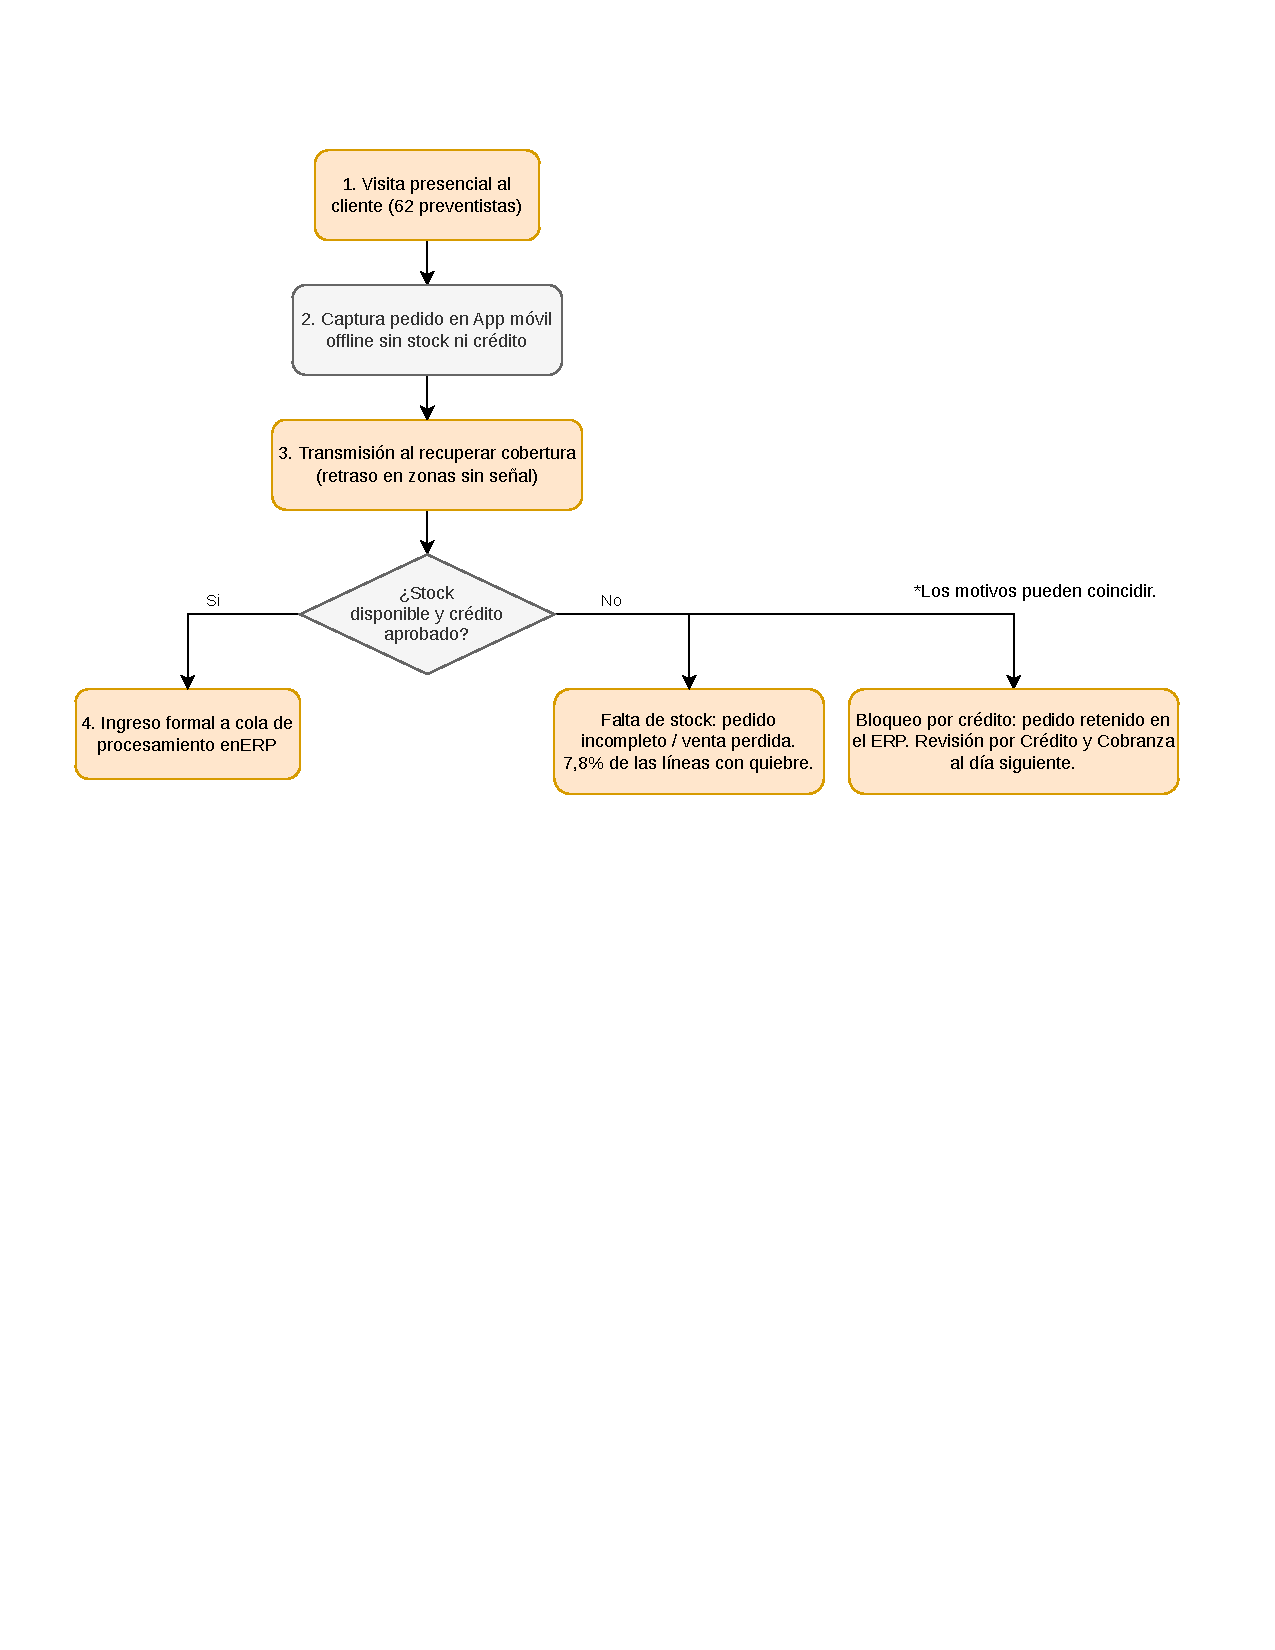
\includegraphics[page=1,trim=32pt 407pt 42pt 68pt,clip,scale=1.15]{figuras/figura 2.1.pdf}
\caption{Proceso de Preventa y Toma de Pedidos AS-IS. Fuente: elaboración propia.}
\label{fig:asis_preventa}
\end{figure}
\end{landscape}

\needspace{9\baselineskip}
\begin{enumerate}
  \item El preventista visita presencialmente al cliente; participan 62 preventistas.
  \item Captura el pedido en una aplicación móvil desconectada, sin visibilidad de stock ni crédito.
  \item Transmite el pedido cuando el dispositivo recupera cobertura; en zonas sin señal, el envío se retrasa hasta encontrarla. La ventana de 17:00 a 20:00 corresponde al regreso y sincronización de la flota, no a la preventa.
  \item El proceso consulta si existe stock disponible y crédito aprobado.
  \item Si la respuesta es afirmativa, el pedido ingresa formalmente a la cola de procesamiento del ERP.
  \item Si la respuesta es negativa, se distinguen dos motivos que pueden coincidir: falta de stock, que produce pedidos incompletos o ventas perdidas y cuyo quiebre afecta al 7,8 \% de las líneas; o bloqueo por crédito, que deja el pedido retenido en el ERP para revisión por Crédito y Cobranza al día siguiente.
\end{enumerate}

La Figura~2.1 muestra que la falla no nace en el ERP, sino antes. El preventista promete sin ver stock ni crédito, y el error recién aparece cuando el pedido llega al sistema. El quiebre se detecta en la preventa, pero lo sufre el cliente en la entrega, porque recibe menos de lo pedido. Hoy no se registra cuántos pedidos quedan retenidos por crédito ni cuánto esperan; es un dato que habrá que medir.

\subsubsection{Proceso 2: Recepción de Mercadería y Control de Lotes AS-IS}

En la Figura~2.2 se ilustra el registro de recepciones en los muelles de los centros de distribución al descargar los envíos de los 180 proveedores.

\needspace{9\baselineskip}
\begin{enumerate}
  \item Arriba un camión al muelle del centro de distribución; la operación se relaciona con 180 proveedores.
  \item Se descargan y cuentan físicamente los bultos en el andén.
  \item La recepción se registra manualmente en una planilla física o guía en papel.
  \item El proceso consulta si lote y vencimiento fueron digitados en el sistema.
  \item Si la respuesta es afirmativa, la mercadería queda con lote registrado.
  \item Si la respuesta es negativa, queda comprometida la trazabilidad sanitaria; 41 \% de las recepciones del producto involucrado en el retiro no tenía lote registrado.
\end{enumerate}

\renewcommand{\thefigure}{2.2}
\begin{figure}[H]
\centering
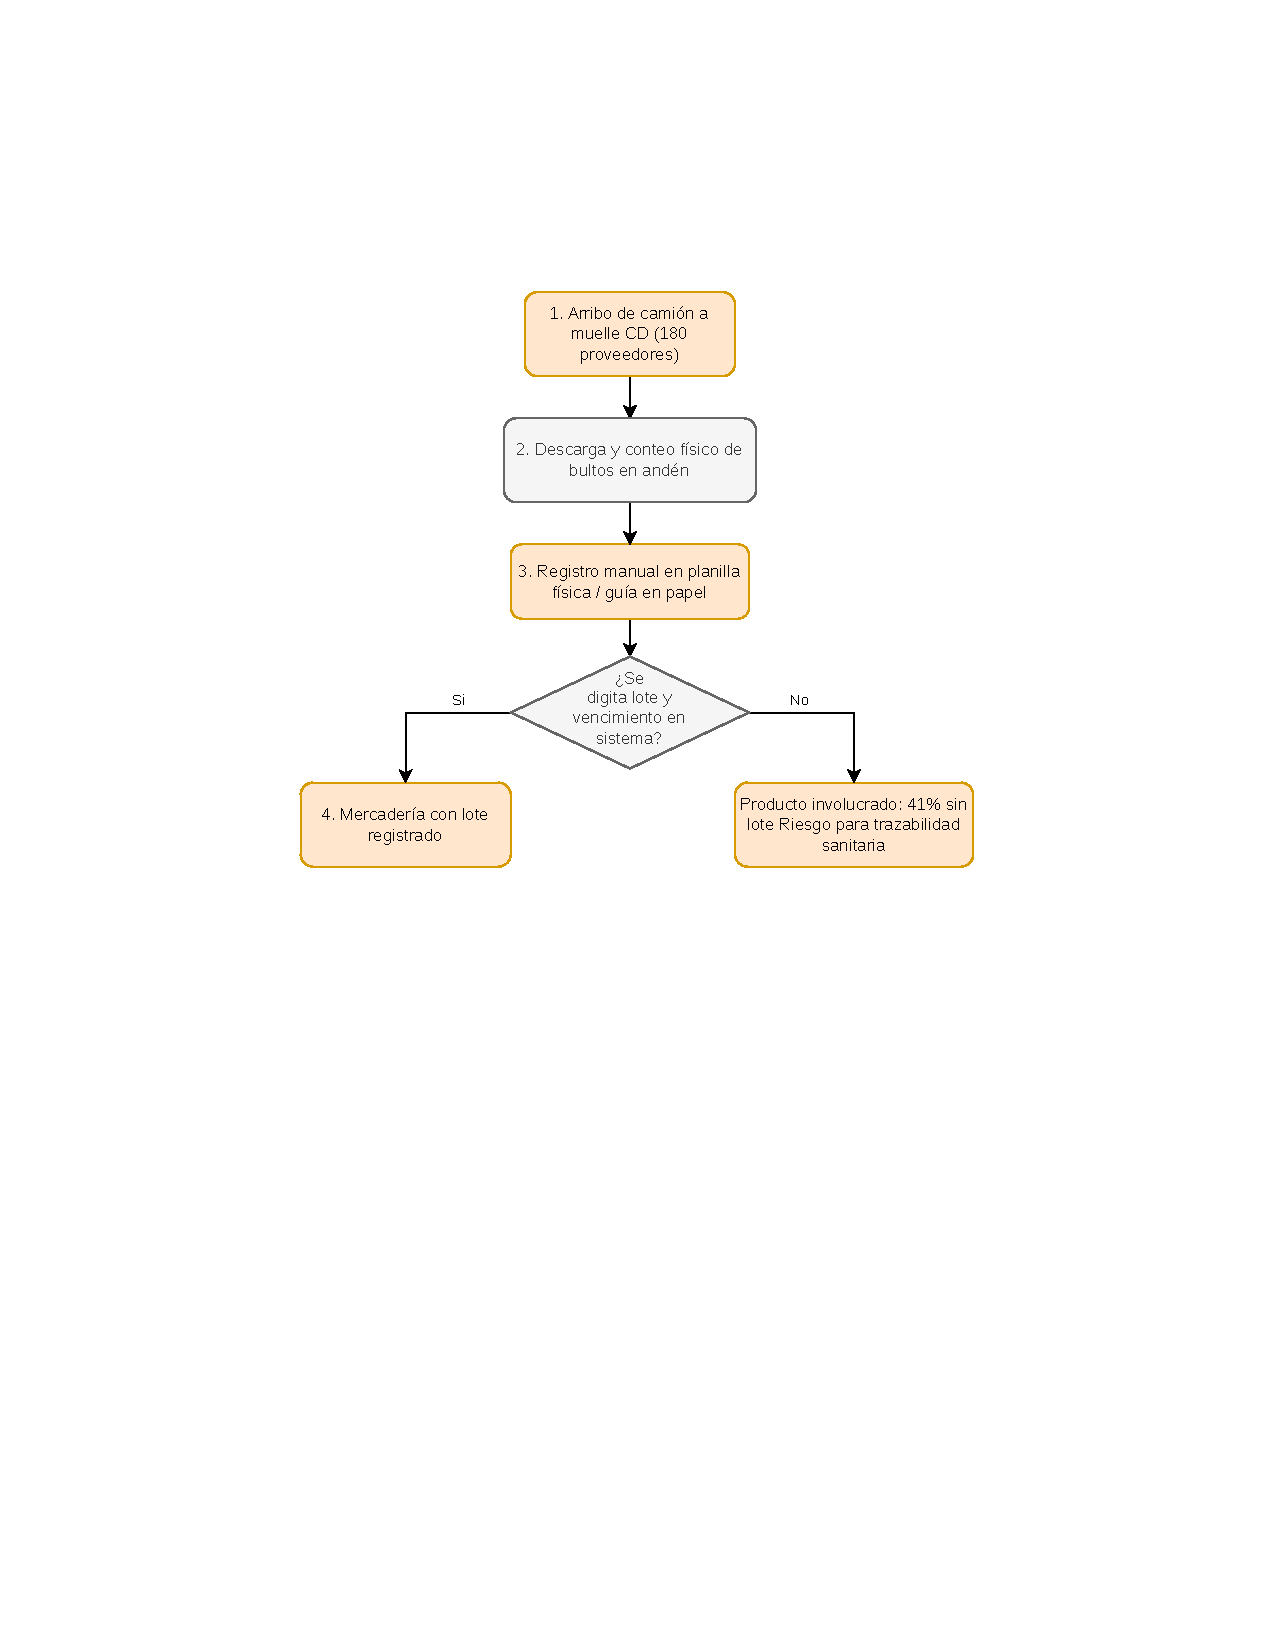
\includegraphics[page=1,trim=140pt 372pt 141pt 136pt,clip,scale=1.24]{figuras/figura 2.2.pdf}
\caption{Proceso de Recepción de Mercadería y Control de Lotes AS-IS. Fuente: elaboración propia.}
\label{fig:asis_recepcion}
\end{figure}

En la Figura~2.2 se ve que el lote se pierde en el paso 3, en el andén, y ningún paso posterior lo recupera: bodega, preparación y despacho mueven la mercadería sin saber de qué lote es. Por eso el retiro de marzo tomó 9 días: hubo que reconstruir con papeles y memoria lo que nunca se registró al recibir. El 41 \% corresponde solo al producto del retiro; cuánto falta en las demás recepciones se desconoce (Anexo~2.2, SP-03) y es lo primero que conviene medir.

\subsubsection{Proceso 3: Preparación de Pedidos y Cross-Docking AS-IS}

La operación de las tres plataformas de cross-docking (Curicó, Chillán y Los Ángeles) se detalla en la Figura~2.3, según la descripción del caso.

\renewcommand{\thefigure}{2.3}
\begin{figure}[H]
\centering
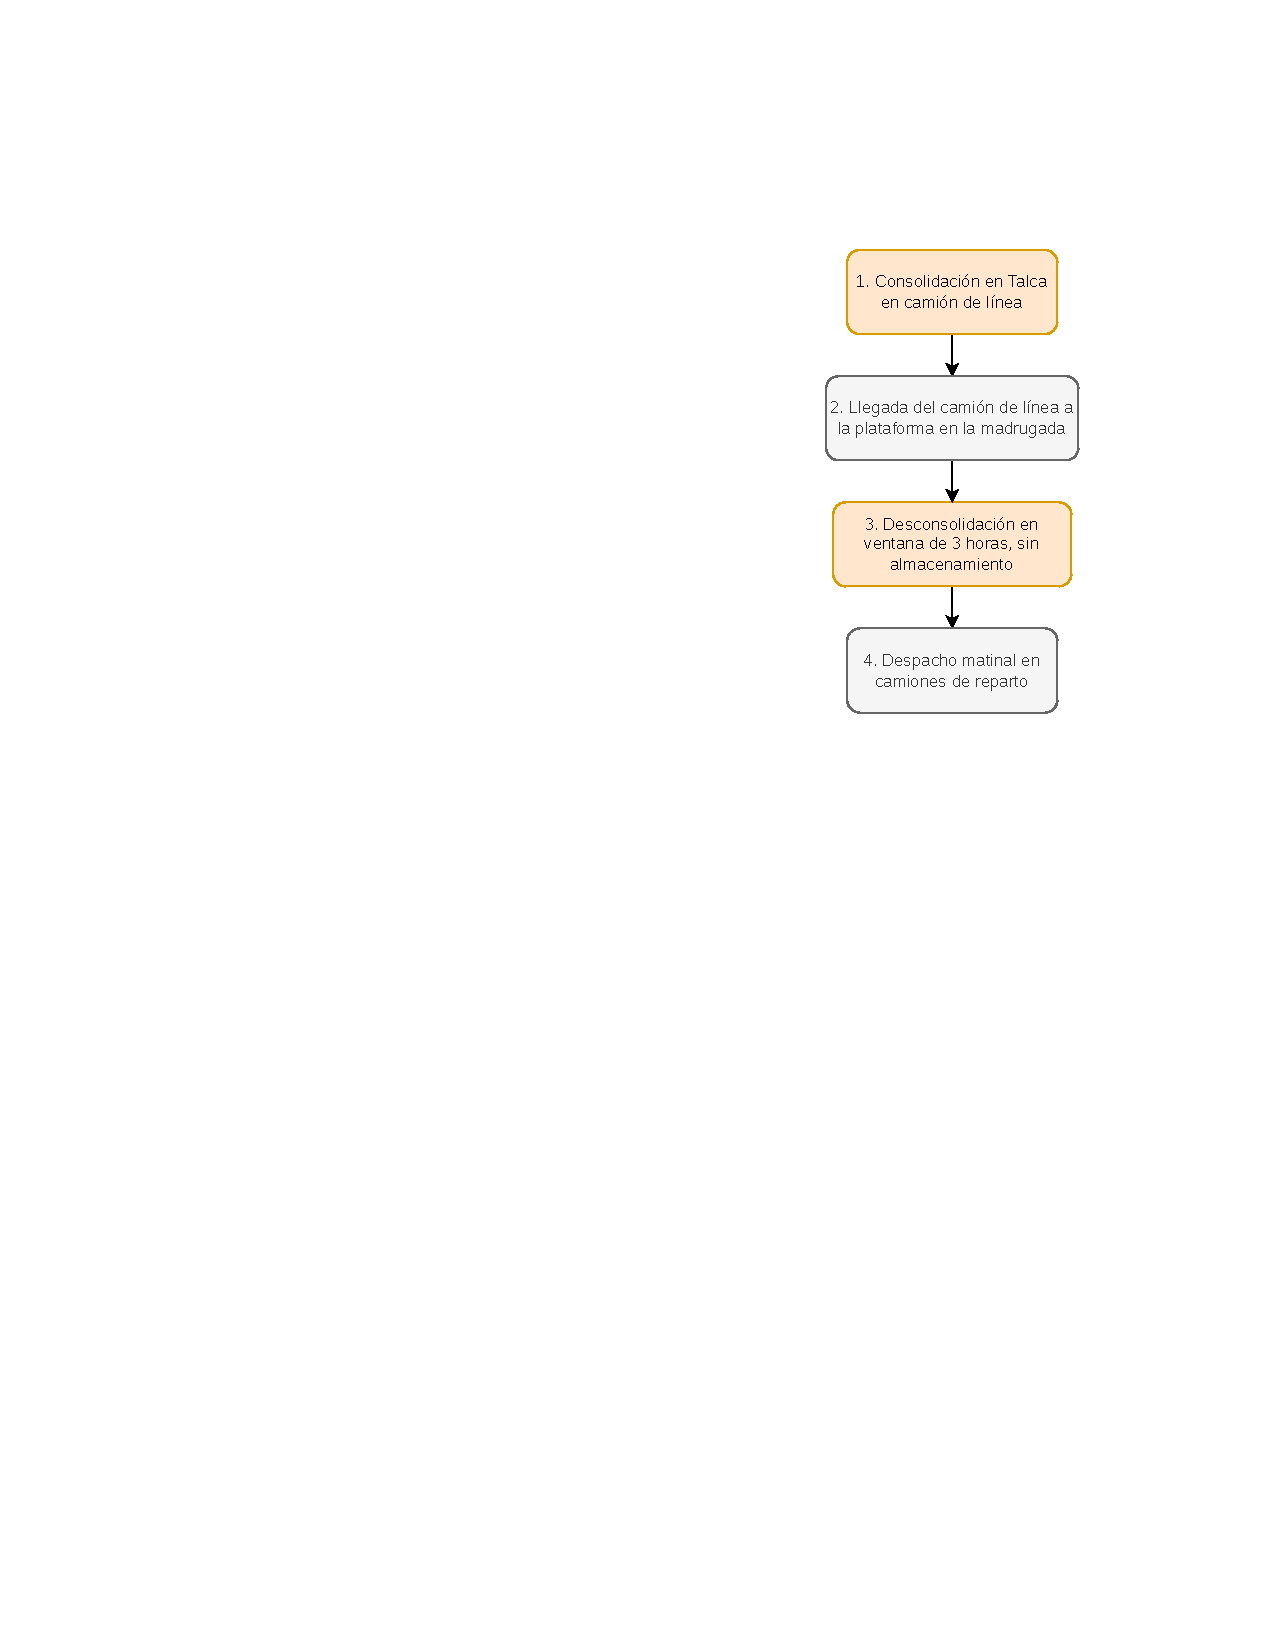
\includegraphics[page=1,trim=392pt 446pt 90pt 116pt,clip,scale=1.14]{figuras/figura 2.3.pdf}
\caption{Proceso de Preparación y Cross-Docking AS-IS. Fuente: elaboración propia.}
\label{fig:asis_crossdocking}
\end{figure}

\needspace{9\baselineskip}
\begin{enumerate}
  \item En Talca se consolida la carga de cada plataforma en el camión de línea.
  \item El camión de línea llega a la plataforma en la madrugada.
  \item La carga se desconsolida en una ventana de operación de tres horas, sin almacenamiento y con personal reducido.
  \item La carga se despacha en la mañana en los camiones de reparto.
\end{enumerate}

Las plataformas operan con conectividad únicamente por red móvil y sin control de inventario (Distribuidora Puelche S.A., 2026c, cap. 6, pp. 10--11, y sección 4.2, p. 7).

La Figura~2.3 tiene cuatro tramos, pero ninguno deja hora registrada: no se sabe cuándo sale el camión de Talca, cuándo llega a la plataforma ni cuánto dura la desconsolidación. Sin esas marcas, las 16 horas no se pueden repartir entre consolidación, viaje, espera o descarga. La compañía sospecha de la consolidación en Talca, pero no hay datos que lo confirmen ni que lo desmientan, así que se trata como hipótesis (Anexo~2.2, SP-02) hasta medir cada tramo.

\subsubsection{Proceso 4: Planificación de Rutas AS-IS}

El proceso de diagramación de despachos y asignación de vehículos se ilustra en la Figura~2.4.

\needspace{9\baselineskip}
\begin{enumerate}
  \item Los pedidos confirmados quedan disponibles para planificación entre las 15:00 y las 18:30 horas.
  \item Los datos se exportan manualmente a planillas Excel, sin interfaz directa.
  \item Las rutas se diagraman manualmente con el conocimiento tácito del planificador.
  \item Se imprimen las hojas de ruta y guías para la tripulación.
  \item El despacho opera con rutas rígidas y subóptimas y alcanza 68 \% de ocupación.
\end{enumerate}

\renewcommand{\thefigure}{2.4}
\begin{figure}[H]
\centering
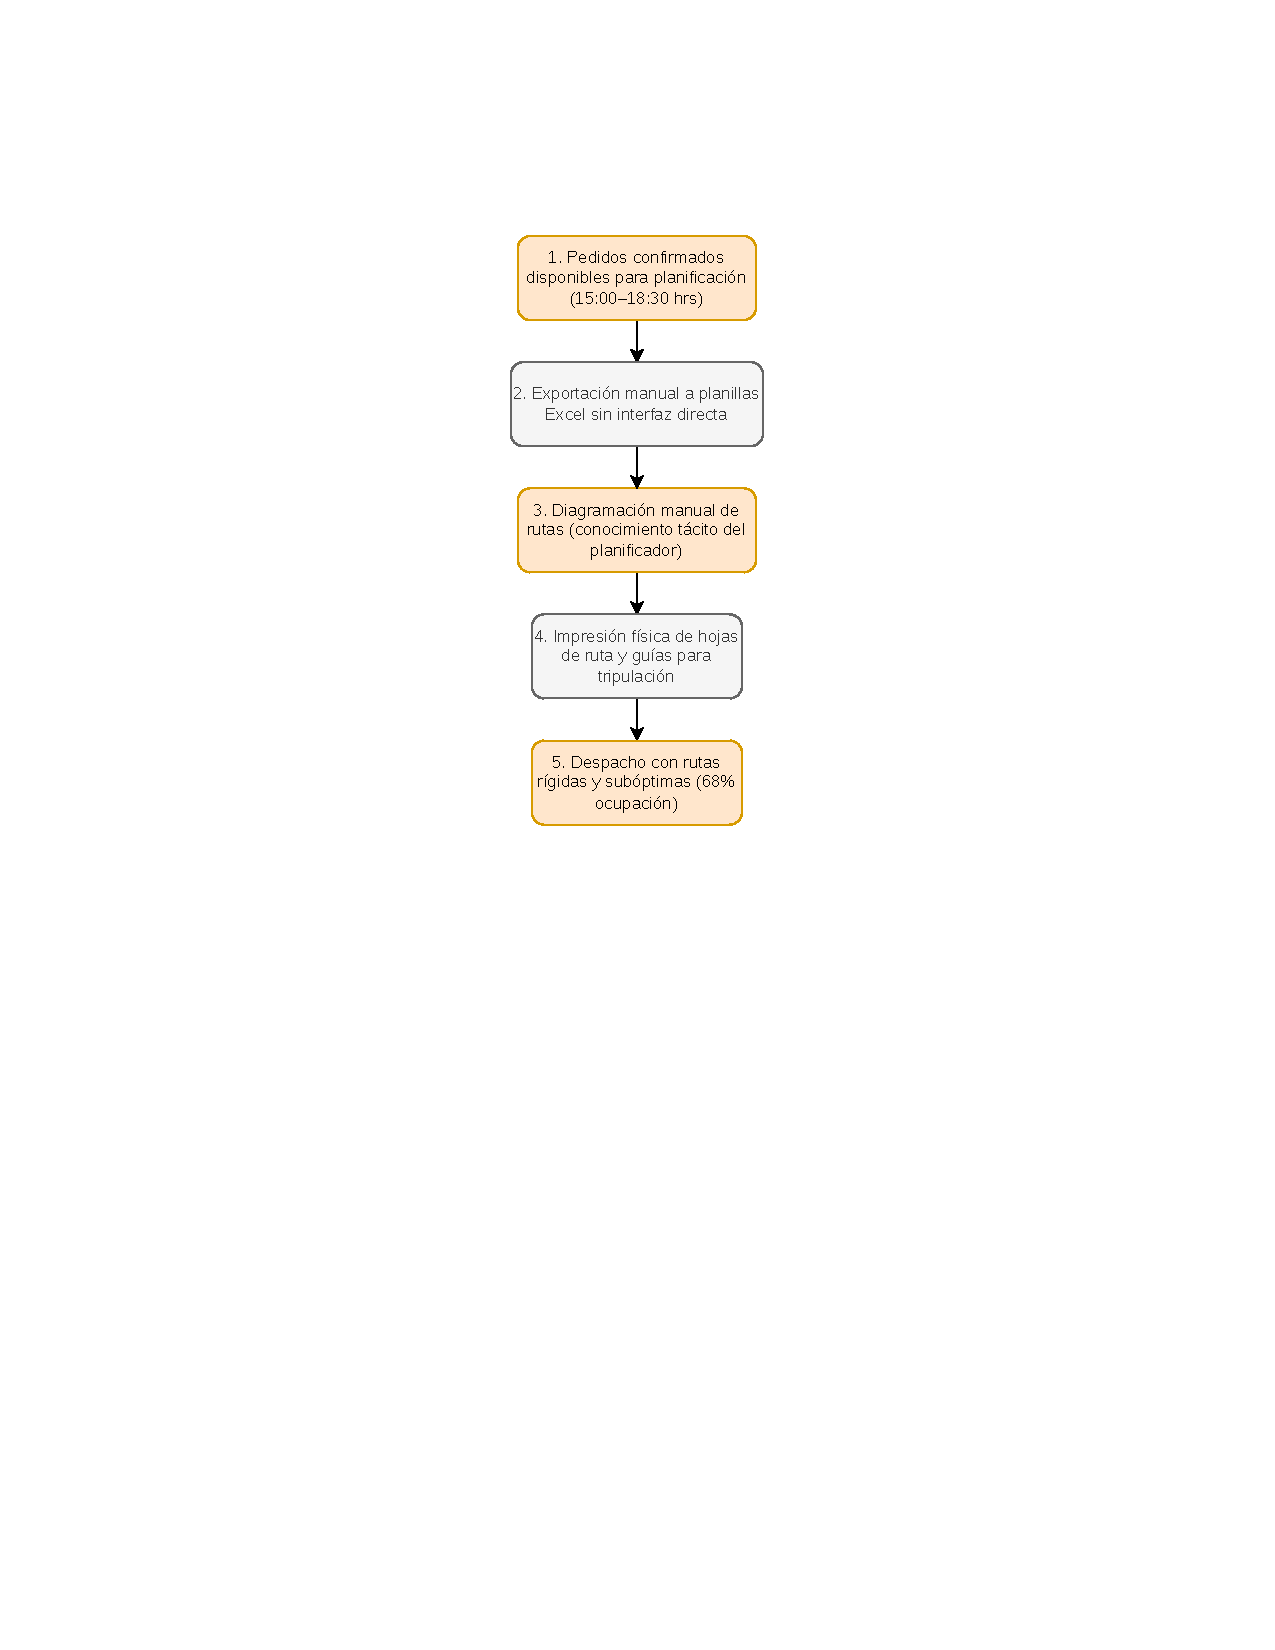
\includegraphics[page=1,trim=241pt 392pt 242pt 109pt,clip,scale=1.14]{figuras/figura 2.4.pdf}
\caption{Proceso de Planificación de Rutas AS-IS. Fuente: elaboración propia.}
\label{fig:asis_planificacion}
\end{figure}

El cuello de botella de la Figura~2.4 es una persona. El planificador tarda 3,5 horas diarias en armar las rutas con una planilla de once hojas que solo él entiende, y cuando sale de vacaciones el cumplimiento de entrega cae entre seis y nueve puntos (Distribuidora Puelche S.A., 2026c, sección 4.4, p. 8). La ocupación de 68 \%, que baja a 41 \% en los días de menor carga, se explica porque el método manual no permite probar alternativas, no por falta de esfuerzo. Si se jubila sin dejar sus reglas por escrito, ese conocimiento se va con él.

\subsubsection{Proceso 5: Reparto y Entrega AS-IS}

La interacción en la última milla entre los camiones de reparto y los puntos de destino se presenta en la Figura~2.5.

\needspace{9\baselineskip}
\begin{enumerate}
  \item El camión sale a ruta durante la ventana de despacho de 05:30 a 07:00 horas.
  \item Arriba al local comercial, ya sea almacén o cliente de food service.
  \item El proceso consulta si el local está abierto y el cliente está conforme.
  \item Si la respuesta es afirmativa, el cliente firma físicamente la guía de despacho.
  \item Si el local está cerrado, el conductor decide si vuelve más tarde, deja el pedido con el negocio vecino o se lo lleva de vuelta; no existe una regla escrita. Si el cliente rechaza un producto, el conductor lo anota en la guía y se lo lleva de vuelta.
\end{enumerate}

\renewcommand{\thefigure}{2.5}
\begin{landscape}
\begin{figure}[p]
\centering
%  La exportación de draw.io reparte el diagrama en dos páginas: la segunda
%  contiene el borde derecho de la última caja. Se unen sin alterarlas.
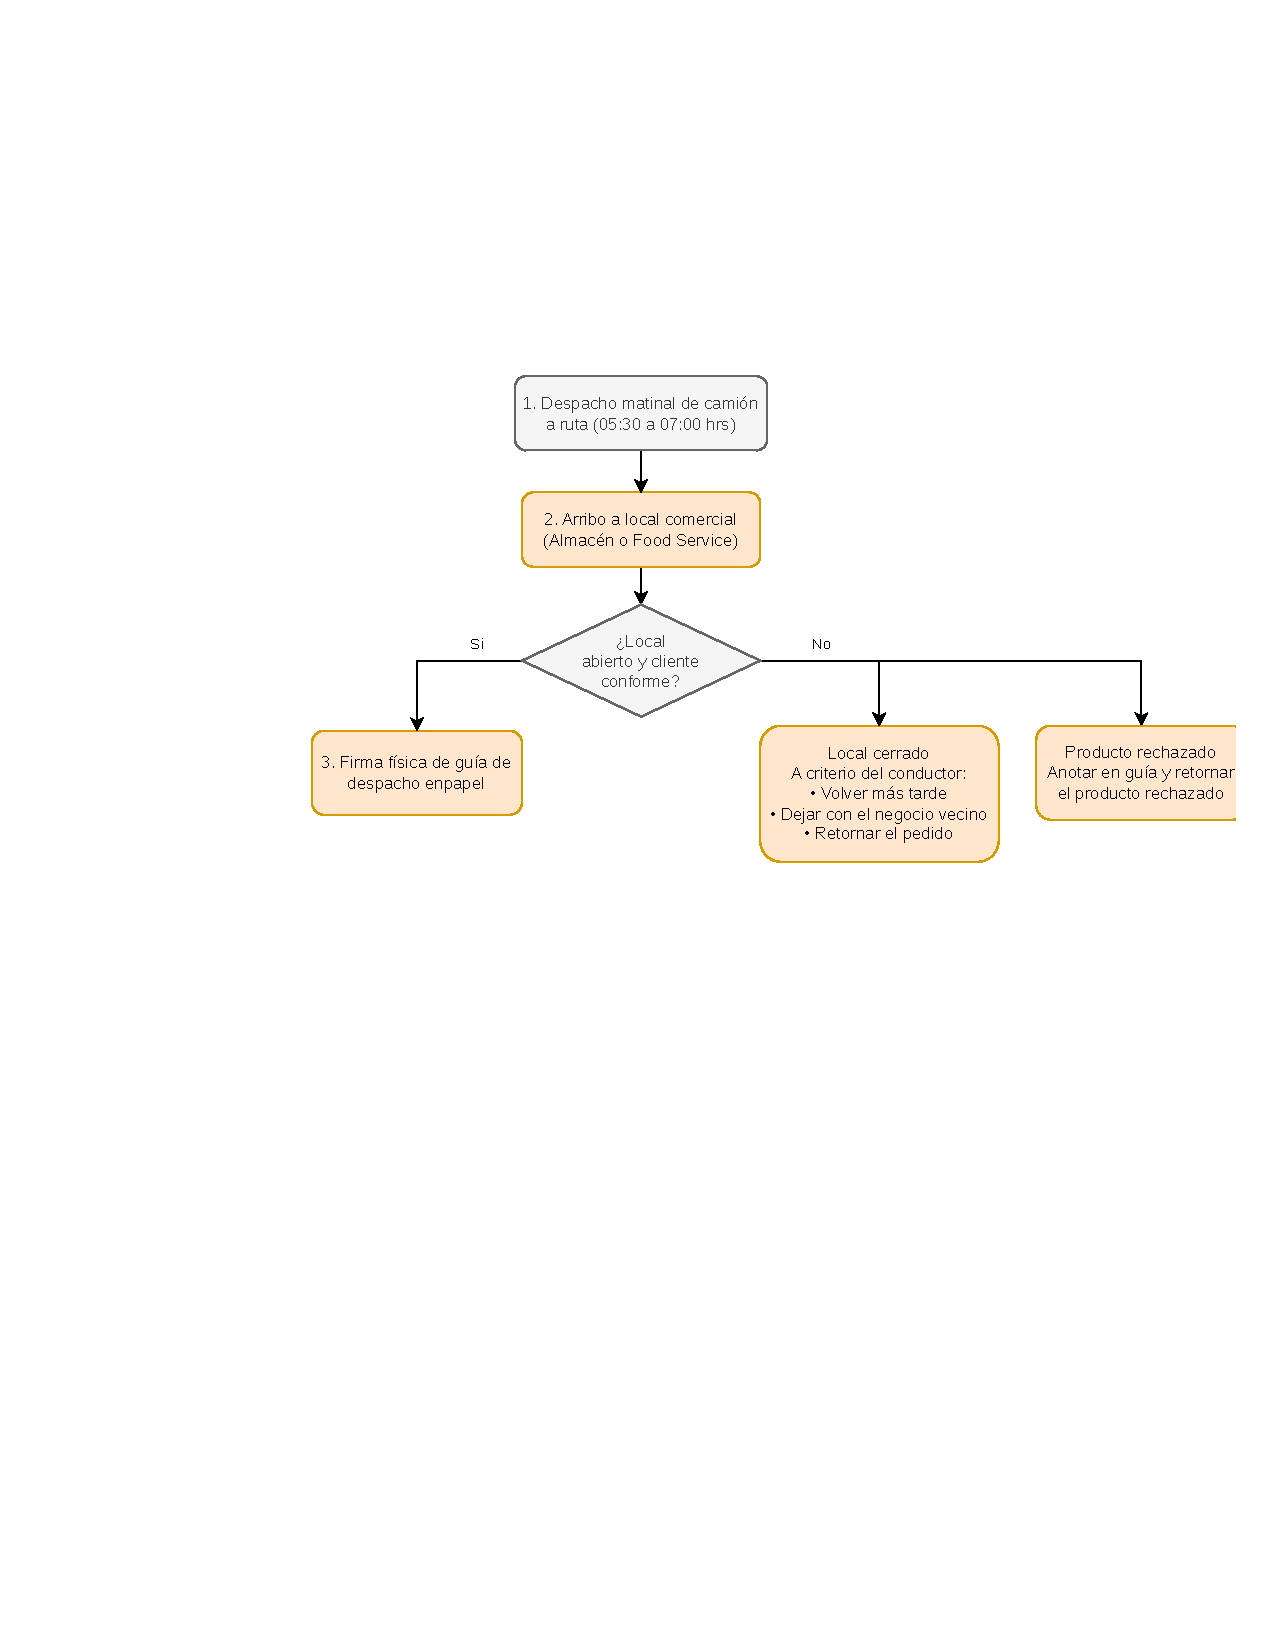
\includegraphics[page=1,trim=146pt 374pt 20.2pt 176pt,clip,scale=1.24]{figuras/figura 2.5.pdf}%
\includegraphics[page=2,trim=20.02pt 374pt 582.1pt 176pt,clip,scale=1.24]{figuras/figura 2.5.pdf}
\caption{Proceso de Reparto y Entrega AS-IS. Fuente: elaboración propia.}
\label{fig:asis_reparto}
\end{figure}
\end{landscape}

En la Figura~2.5, la entrega es donde se cierran o se rompen los procesos anteriores. Como no hay regla escrita para el local cerrado, cada conductor resuelve a su manera y la reentrega no queda registrada con su causa. El retorno de mercadería tampoco equivale siempre a una reentrega. La única prueba de entrega es la guía firmada en papel: si se pierde (1,1 \% al mes), aclarar un reclamo toma en promedio 12 días.

La tasa de reentregas es del 4,2 \% sobre el total de entregas (Distribuidora Puelche S.A., 2026c, cap. 7, tabla 7.1, p. 11). Aplicada a las aproximadamente 1.400 entregas de un día hábil normal, equivale a unas 59 reentregas diarias (1.400 $\times$ 0,042 = 58,8). Esta estimación está condicionada al supuesto SP-01 del Anexo~2.2, que requiere validar la aplicación de la tasa al volumen diario y la correspondencia de cada reentrega con una entrega. La cifra no representa la cantidad de retornos de mercancía al centro de distribución.

\subsubsection{Proceso 6: Rendición y Cobranza AS-IS}

Por último, la liquidación de valores cobrados en efectivo se esquematiza en la Figura~2.6.

\renewcommand{\thefigure}{2.6}
\begin{figure}[H]
\centering
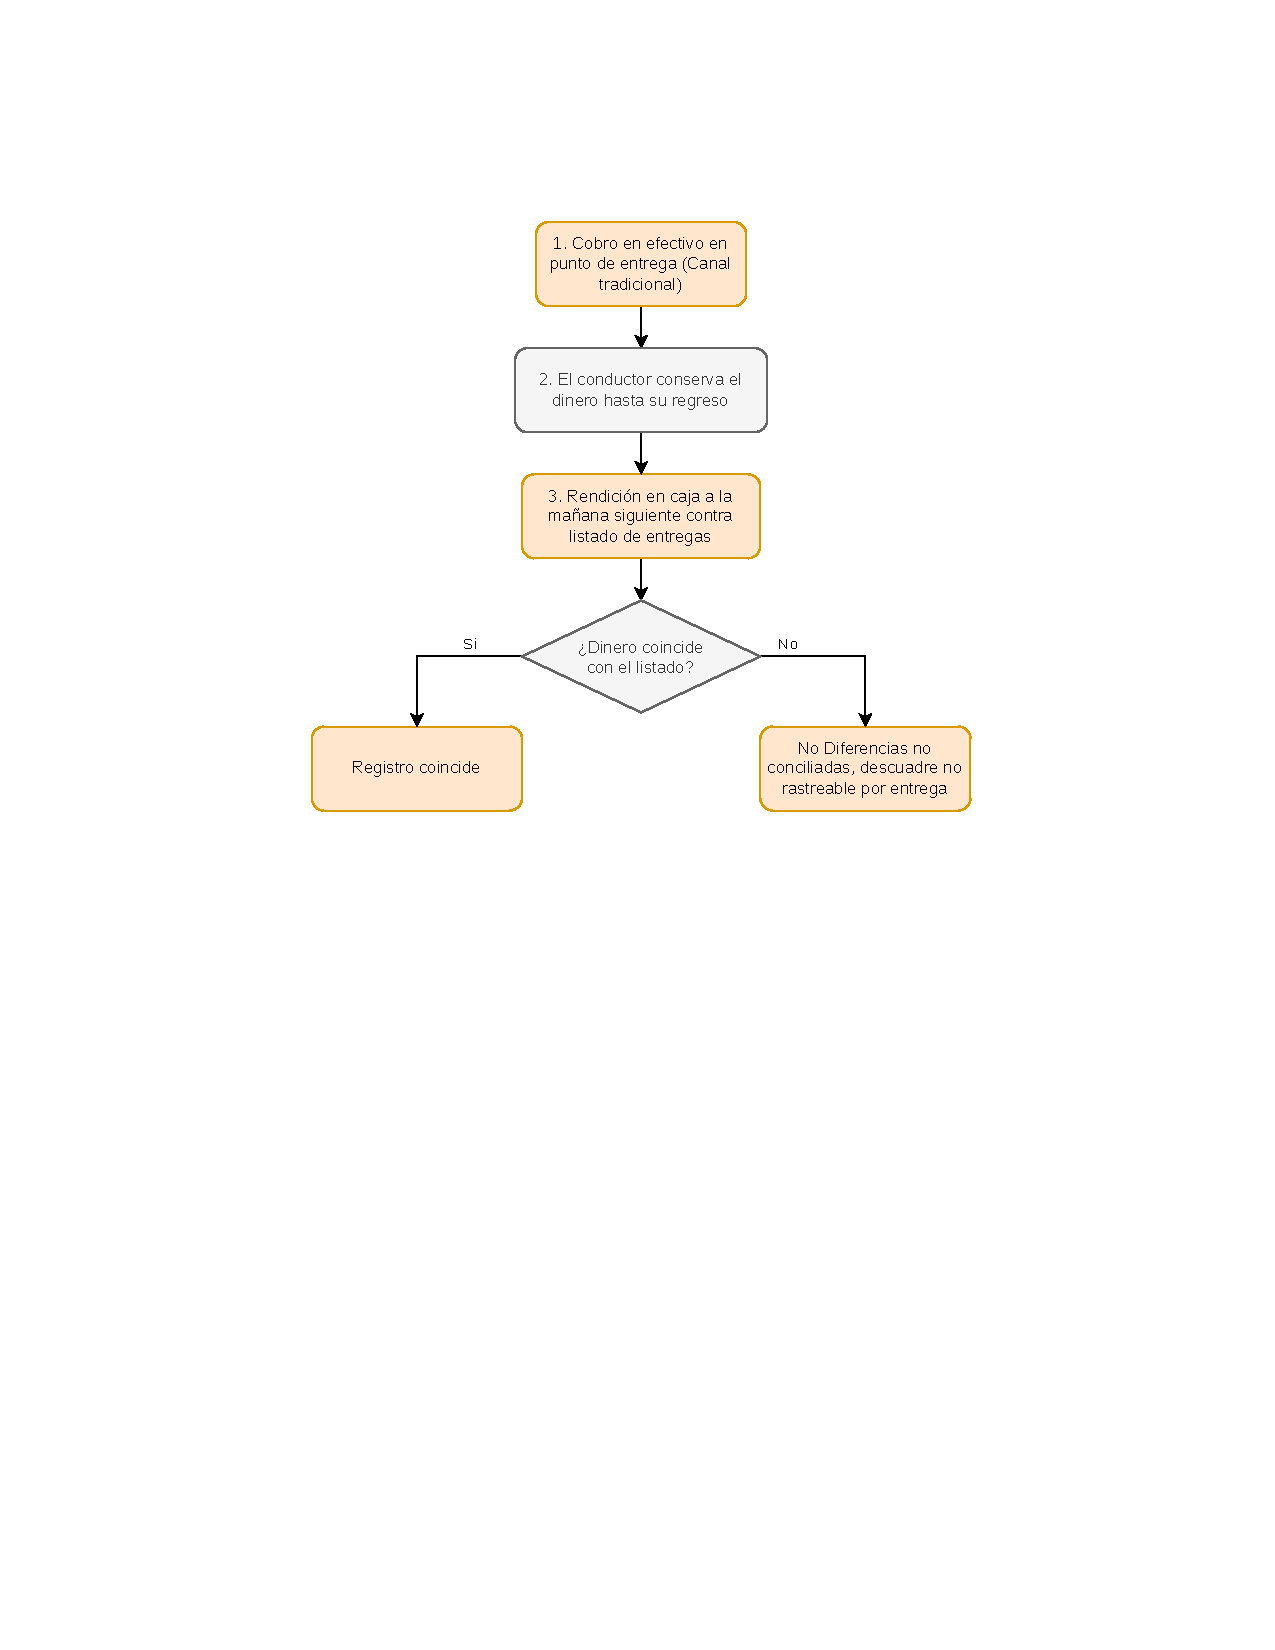
\includegraphics[page=1,trim=146pt 399pt 142pt 103pt,clip,scale=1.24]{figuras/figura 2.6.pdf}
\caption{Proceso de Rendición y Cobranza AS-IS. Fuente: elaboración propia.}
\label{fig:asis_rendicion}
\end{figure}

\needspace{9\baselineskip}
\begin{enumerate}
  \item Se cobra en efectivo contra entrega; el 38 \% de las ventas del canal tradicional se cobra así y el resto se factura a 30 días.
  \item El conductor conserva el dinero hasta su regreso.
  \item La rendición se realiza a la mañana siguiente en caja, contando el dinero contra el listado de entregas del día anterior.
  \item La caja consulta si el dinero contado coincide con el listado de entregas al contado del día anterior.
  \item Si coincide, se registra sin inconvenientes.
  \item Si la respuesta es negativa, quedan diferencias no conciliadas y no es posible rastrear el descuadre por entrega.
\end{enumerate}

La Figura~2.6 muestra un desfase: el descuadre ocurre en la calle, pero se descubre a la mañana siguiente en la caja, cuando ya no se sabe en qué entrega se produjo. Por eso los \$ 4,2 millones mensuales de diferencia siguen sin investigar. El problema no es que falte control en la caja, sino que el cobro no queda unido a su entrega en el momento en que ocurre.

Leídos juntos, los seis procesos repiten un mismo patrón: el dato nace en terreno, se anota en papel o queda en la memoria de alguien, y se reconstruye después, cuando ya no se puede verificar. Así se pierden el lote en la recepción, la causa del faltante en la preventa, la evidencia en la guía y el origen del descuadre en la rendición. Cada pérdida afecta al proceso siguiente, y por eso los tres problemas de la sección 2.2.1 aparecen juntos.

\section{Actores y Grupos de Interés}

El éxito del proyecto depende de alinear a los 19 actores que conforman el ecosistema de Distribuidora Puelche S.A. Cada uno posee incentivos, niveles de poder y resistencias particulares frente a la automatización de procesos.

%  La Tabla 2.2 no se corta entre páginas (Aclaraciones §5).
\needspace{0.42\textheight}
Para analizar su nivel de influencia e interés, la Tabla~2.2 agrupa a los 19 actores en cinco grupos y registra la tensión principal de cada uno.

\renewcommand{\thetable}{2.2}
\begin{tablalafrox}{Actores agrupados por influencia e interés. Fuente: elaboración propia a partir de Distribuidora Puelche S.A. (2026c, caps. 2 y 8, pp. 4--5 y 13--17).}%
  {tab:2-2}%
  {F{0.34} G{0.14} G{0.12} Y}%
  {\cab{Grupo y actores} & \cab{Influencia} & \cab{Interés} & \cab{Tensión principal}}
  Dirección: gerenta general, gerente comercial y gerente de finanzas & Muy alta & Muy alto & Promesa de 24 horas frente a la capacidad real y condiciones de 2029. \\
  Jefaturas: operaciones, calidad, bodega, TI y planificador de rutas & Alta & Muy alto & Brecha de 16 horas, lotes sin registro y planificador que se jubila. \\
  Terreno: 62 preventistas, 84 conductores y peonetas, unos 160 conductores externos, 120 preparadores y sindicato & Alta & Alto & Venta sin stock ni crédito y objeción a cámaras y GPS. \\
  Clientes: 11.600 tradicionales, 2.100 de \textit{food service} y 500 del canal moderno & Muy alta & Alto & OTIF de 82,4 \% sin poder exigirles internet ni pago electrónico. \\
  Externos: 180 proveedores, 10 transportistas y autoridad sanitaria & Media-alta & Alto & Rotulado de lote, rotación de conductores y registro de temperatura. \\
\end{tablalafrox}

La Tabla~2.2 muestra que el interés no distingue a los grupos: todos tienen interés alto o muy alto, porque el proyecto cambia su trabajo diario. La diferencia está en la influencia. Dirección y clientes tienen influencia muy alta: la primera decide las prioridades y la segunda define si la empresa conserva su venta. Jefaturas y personal de terreno influyen por otra vía: sin su cooperación la operación no cambia, aunque el sistema funcione. Proveedores, transportistas y autoridad influyen menos en el día a día, pero imponen condiciones externas. Por eso los cuatro primeros grupos requieren una gestión cercana, y el quinto, información oportuna y acuerdos formales.

El mayor riesgo de resistencia está en el personal de terreno: el sindicato ya objetó las cámaras en cabina y el uso del GPS para controlar la jornada, y el planificador concentra un conocimiento que nadie más tiene. El catálogo nominal de los 19 actores, con su estrategia de participación, está en el Anexo~2.3, y el Subdocumento 3 desarrolla cómo se obtiene su apoyo.

\section[Resumen de Requerimientos, Supuestos, Exclusiones y Restricciones]{Resumen de Requerimientos, Supuestos, Exclusiones\\ y Restricciones}

Esta sección resume lo que el CLIENTE requiere, los supuestos que formula LafroX y las exclusiones y restricciones del caso; el detalle está en los Anexos~2.1 a 2.3.

\subsection{Resumen y análisis de requerimientos del cliente}

A partir del análisis del problema y de las entrevistas del caso (Distribuidora Puelche S.A., 2026c, cap. 8, pp. 13--17), el cliente exige una solución que satisfaga un catálogo integral de requerimientos funcionales y no funcionales. Los principales ejes funcionales demandados abarcan:

\begin{itemize}
  \item \textbf{Preventa y comercialización:} El preventista necesita conocer stock y crédito al tomar el pedido y seguir trabajando un turno completo sin señal, sin que ningún pedido se pierda ni se duplique.
  \item \textbf{Gestión de bodegas y trazabilidad de lotes:} Todo producto que lo requiera debe quedar con lote y vencimiento desde su recepción, salir en orden de vencimiento, también en la cámara a $-$22\,°C, y permitir identificar a los clientes afectados por un lote en menos de 2 horas.
  \item \textbf{Despacho y última milla:} Rutas que respeten la promesa segmentada y las ventanas de servicio, evidencia de cada entrega disponible el mismo día y acuse de recibo válido de la Guía de Despacho Electrónica.
  \item \textbf{Conciliación financiera:} Cada cobro en efectivo debe quedar asociado a su entrega, y toda diferencia de rendición debe explicarse el mismo día con causal y responsable.
\end{itemize}

A estos ejes se suman condiciones no funcionales de las Bases Técnicas Transversales, como la disponibilidad mensual de 99,95 \% por componente de infraestructura y de 99,9 \% para la transacción de negocio de extremo a extremo (Distribuidora Puelche S.A., 2026b, cap. 7, sección 7.2, pp. 17--18). El catálogo completo y priorizado de requerimientos funcionales y no funcionales se detalla en el Anexo~2.1.

\subsection{Supuestos de ingeniería formulados por LafroX}

Para diseñar una propuesta técnicamente sólida y exenta de contingencias imprevistas, LafroX formula un conjunto de supuestos propios de ingeniería, deslindándolos formalmente de las restricciones impuestas por las bases. El detalle, con fundamento, impacto y mecanismo de validación, se presenta en el Anexo~2.2.

\subsection{Exclusiones y restricciones no negociables}

Complementariamente, la Tabla~2.3 sintetiza cinco de las doce restricciones del caso, con los mismos códigos del Anexo~2.2. La inmutabilidad del canal tradicional y la prohibición de intervenir sistemas del 1 al 25 de septiembre, durante todo diciembre y en los tres primeros días hábiles de cada mes condicionan la propuesta de dos formas. Obligan a que la operación de terreno no dependa del sistema central. También obligan a programar despliegues y pasos a producción fuera de esos períodos (Distribuidora Puelche S.A., 2026c, cap. 10, pp. 19--20, y sección 13.3, p. 23). El inventario íntegro de exclusiones y restricciones se encuentra en el Anexo~2.2.

\renewcommand{\thetable}{2.3}
\begin{tablalafrox}{Síntesis de restricciones no negociables del caso. Fuente: Distribuidora Puelche S.A. (2026c, cap. 10, pp. 19--20); detalle en el Anexo 2.2.}%
  {tab:2-3}%
  {F{0.11} F{0.30} Y}%
  {\cab{Código} & \cab{Restricción} & \cab{Condición que impone}}
  R-04 & ERP como registro contable único & El ERP no se sustituye y sigue siendo el único emisor de documentos tributarios. \\
  R-05 & Canal tradicional sin cambios & A los 11.600 almacenes no se les exige internet, dispositivo propio ni pago electrónico. \\
  R-08 & Ventanas de congelamiento & No se interviene del 1 al 25 de septiembre, en diciembre ni en los tres primeros días hábiles de cada mes. \\
  R-10 & Privacidad laboral & El sindicato objetó las cámaras en cabina y el control de jornada por GPS. \\
  R-12 & Validez de los documentos tributarios & La guía de despacho electrónica y su acuse tienen efectos legales que no se pueden comprometer. \\
\end{tablalafrox}

Las cinco restricciones de la Tabla~2.3 limitan la propuesta en tres planos. En terreno, R-05 y R-10 exigen generar la evidencia de entrega y cobro con recursos de Puelche y respetar los límites al uso de cámaras y GPS. En la integración, R-04 y R-12 mantienen al ERP como emisor de documentos tributarios. En el calendario, R-08 condiciona las intervenciones y los pasos a producción a las ventanas permitidas.

\section*{Referencias}
\addcontentsline{toc}{section}{Referencias}

Las fuentes citadas en este documento se listan a continuación en formato APA 7.ª edición.

\begin{itemize}
  \item Distribuidora Puelche S.A. (2026a). \textit{Bases Administrativas de Licitación N° TFEP-01/2026: Contratación de Solución Integral de Software y Servicios de Operación}.
  \item Distribuidora Puelche S.A. (2026b). \textit{Bases Técnicas Transversales de Licitación N° TFEP-01/2026}.
  \item Distribuidora Puelche S.A. (2026c). \textit{Bases Técnicas -- Logística: trazabilidad, promesa de entrega y costo de servir en una distribuidora de consumo masivo}.
  \item GS1 Chile. (2020). \textit{Estándares de Identificación y Trazabilidad Logística GS1: Guía de Aplicación para Consumo Masivo y Retail} (Versión 20.0). GS1.
  \item Ley N.º 21.719. (2024, 13 de diciembre). \textit{Regula la protección y el tratamiento de los datos personales y crea la Agencia de Protección de Datos Personales}. Diario Oficial de la República de Chile. \url{https://www.bcn.cl/leychile/navegar?idNorma=1209272}
  \item Ministerio de Salud. (1996). \textit{Decreto Supremo N° 977: Aprueba Reglamento Sanitario de los Alimentos}. Diario Oficial de la República de Chile.
  \item Ministerio del Trabajo y Previsión Social. (2002). \textit{Código del Trabajo de la República de Chile: Artículo 25 bis sobre jornada especial de transporte de carga}. Edición oficial.
  \item Servicio de Impuestos Internos. (2024). \textit{Manual de Procedimientos y Requisitos de Documentos Tributarios Electrónicos (DTE)}. SII Chile.
\end{itemize}

\section*{Declaración de uso de IA}
\addcontentsline{toc}{section}{Declaración de uso de IA}

La Tabla~\ref{tab:2-4} declara el uso asistido de herramientas de inteligencia artificial en la elaboración del presente subdocumento.

\renewcommand{\thetable}{2.4}
\begin{tablalafrox}{Declaración de uso de IA por sección del Subdocumento 2. Fuente: registro del equipo.}%
  {tab:2-4}%
  {F{0.22} F{0.14} Y G{0.12} G{0.13} F{0.20}}%
  {\cab{Sección} & \cab{Herramienta} & \cab{Finalidad del uso} & \cab{Nivel en texto} & \cab{Nivel en diagramas} & \cab{Revisión humana (quién y qué verificó)}}
  2.1 Resumen Ejec. & Claude / Gemini & Síntesis ejecutiva y estilo formal & Bajo & Ninguno & Alex Aravena (JP): Validación del resumen y propuesta de valor \\
  2.2 Comprensión & Claude / Gemini & Estructuración de los 3 problemas & Bajo & Ninguno & Patricio Henríquez (Gest): Verificación de arbitraje de tensiones \\
  2.3 Dimensionamiento & Claude / Gemini & Descripción estructurada de los 6 flujos AS-IS & Bajo & Medio & Tomás Pérez (Des): Verificación de flujos AS-IS y cálculos \\
  2.4 Actores & Claude / Gemini & Disposición tabular de actores & Bajo & Ninguno & Patricio Henríquez (Gest): Consistencia con catálogo de actores \\
  2.5 Requerimientos & Claude / Gemini & Formato y redacción de supuestos & Bajo & Ninguno & Bastián Trejo (Arq): Deslinde de supuestos vs restricciones \\
  Anexo~2.1 & Claude / Gemini & Maquetación del listado de requerimientos & Bajo & Ninguno & Bastián Trejo (Arq): Coherencia con el catálogo canónico \\
  Anexo~2.2 & Claude / Gemini & Consolidación de decisiones, exclusiones y restricciones & Bajo & Ninguno & Alex Aravena (JP): Cotejo con los capítulos 10, 11 y 16.1 del caso \\
  Anexo~2.3 & Claude / Gemini & Maquetación de actores y sistemas legados & Bajo & Ninguno & Patricio Henríquez (Gest): Cotejo de actores, cifras y sistemas con el caso \\
\end{tablalafrox}

La Tabla~2.4 muestra que la IA se usó como apoyo de síntesis, estructura y formato en cada sección, y que cada fila declara el integrante que revisó esa sección.
